\chapter{Methodology}\label{ch:Methodology}

The final algorithm is split into two phases.
In the first phase, dubbed as the \textit{index search}, given sequences from multiple FASTA/FASTQ files, searches for the key-$k$-mers.
Then, this index is written to disk, and in the second phase it is read again, where the second phase is known as the \textit{color search}.
In this section, the pipeline of both phases are described first.
The two phases bear a lot of similarities, hence these are further expanded upon in the description of the first phase and some of them will be mentioned again without going into detail when describing the second phase.
Later, some additional techniques will be described, which are used in order to massively parallelise and optimise the phases, which are also common between the two of them, but can be described separately from the main pipeline.
With this structure, the reader will get a good idea of how the data flows and also gets familiar with the components, before jumping into more complex optimisations which would be difficult to grasp without context.

\section{Phase 1: Index Search}\label{sec:Phase1}

The first phase is the index search.
In a nutshell, the purpose of this phase is to (a) load the SBWT and key-$k$-mer marks in GPU memory, (b) parse the FASTA/FASTQ files, (c) perform preprocessing on the sequences such as bitpacking and copy the query data over to the GPU, (d) look up the index of each $k$-mer in the SBWT, and lastly (e) traverse the SBWT to the next key-$k$-mer within the GPU, and finally (f) copy the indexes back to main memory from GPU memory and write them to disk.
This section will go through each of these steps and how each step was optimised or adjusted individually to fit the needs of the new objectives.
Appendix~\ref{app:IndexSearchDataStructures} contains a description of the data structures used in this section.


\subsection{Loading the SBWT}

The first step is to load the SBWT and key-$k$-mer marks.
The SBWT format must be an index created by either Themisto\footnote{\url{https://github.com/algbio/themisto}} or SBWT\footnote{\url{https://github.com/algbio/SBWT}}.
The important factors from this index are the four SBWT bitvectors and the value of $k$.
The next step is to build the Poppy data structure for these four bitvectors.
All Poppys are built in parallel, in four separate threads.
The c-map is created after all Poppys have been built, which is just a cumulative sum of the total 1s of the bitvectors which have been scanned when building the Poppys.
Internally, vectors of u64s are used to store everything.
After they are built, the bitvectors and their accompanying Poppys are copied over to the GPU where they will sit until the end of phase 1.

Depending on the value of $d$, which was described as the checkpointing amount for key-$k$-mers, the algorithm may also need to load the key-$k$-mer marks.
If $d=1$, then this is unnecessary, as the algorithm will not need to move to the next key-$k$-mer within the graph, since every $k$-mer will be a key-$k$-mer.
However, if $d \ne 1$, then it will need to load these from disk and into the GPU memory as well.
These are the same size as a layer 3 bitvector for the four SBWT bitvectors.
Hence, if the small memory requirements of Poppy are ignored, it means that the algorithm will need 25\% more GPU memory than without this bitvector, for this phase.
There is no need to create a Poppy for these marks in this phase, since they will simply be used as a boolean map.
Throughout this chapter, some data structures are introduced and they may be difficult to keep track of.
For this reason, they are summarised in Appendix~\ref{app:IndexSearchDataStructures} with another version for their description.

\subsection{FASTA/FASTQ Parsing}

Next is to parse the FASTA/FASTQ files.
A custom-made parser was built for this which was put in its own repository\footnote{\url{https://github.com/CowKeyMan/kseqpp_REad}} and used as an external library for anyone to use separately.
It is called \texit{kseqpp\_REad} as it is built from kseq++, although highly modified, and it only performs reading, whereas kseq++ can do writing as well.
It is inspired by kseq\footnote{\url{https://github.com/attractivechaos/klib/blob/master/kseq.h}} and kseq++\footnote{\url{https://github.com/cartoonist/kseq++}}, the latter of which is simply a rewrite of the former in C++.
These parsers were inspirations because they are extremely fast and can support a mixture of FASTA and FASTQ formats within the same file and can handle multiline sequences as well.
They can also handle line endings with and without a carriage return.

The reason it was opted to create a custom parser, then, is for load balancing purposes.
The data needs to be loaded in batches, since it would not all fit into main memory or GPU memory, as the datasets may be 100s of GB big or even orders of magnitudes bigger.
Furthermore, it is also useful if each batch has the same number of characters.
With kseq, one can only read full sequence by full sequence.
This means that if a single sequence is hypothetically gigabytes large while others are smaller, there may be a large disparity between the batches, and some batches might even overflow memory, causing disk spills or GPU overflows which would lead to incorrect results or crashes.
Furthermore, kseq++ would produce a vector of strings.
This means that the memory would be fractured in memory, so an extra step would be necessary to copy all the characters to a contiguous vector.

The custom parser, kseqpp\_REad, on the other hand, takes as inputs the file to be read, the maximum characters, and the maximum number of individual sequences it can start reading before returning the batch.
Then, it returns the characters in a single character vector with an accompanying u64 vector where the breaks in the character vector are, called the \textit{chars\_before\_newline}, which is cumulative.
Multiple files are also allowed to be processed within the same batch.
Thus, another u64 vector called the \textit{newlines\_before\_newfile} tells the algorithm where the file breaks should happen, which is also cumulative.
The last u64 of the cumulative vectors is always the maximum u64, which represents infinity, since there will no longer be any breaks.
The choice of the number of maximum characters and sequences per batch is discussed later on in this chapter.
Figure~\ref{fig:FastaqParser} shows an example of parsing a file and what the resulting vectors are.

\begin{figure}[t]
  \centering
  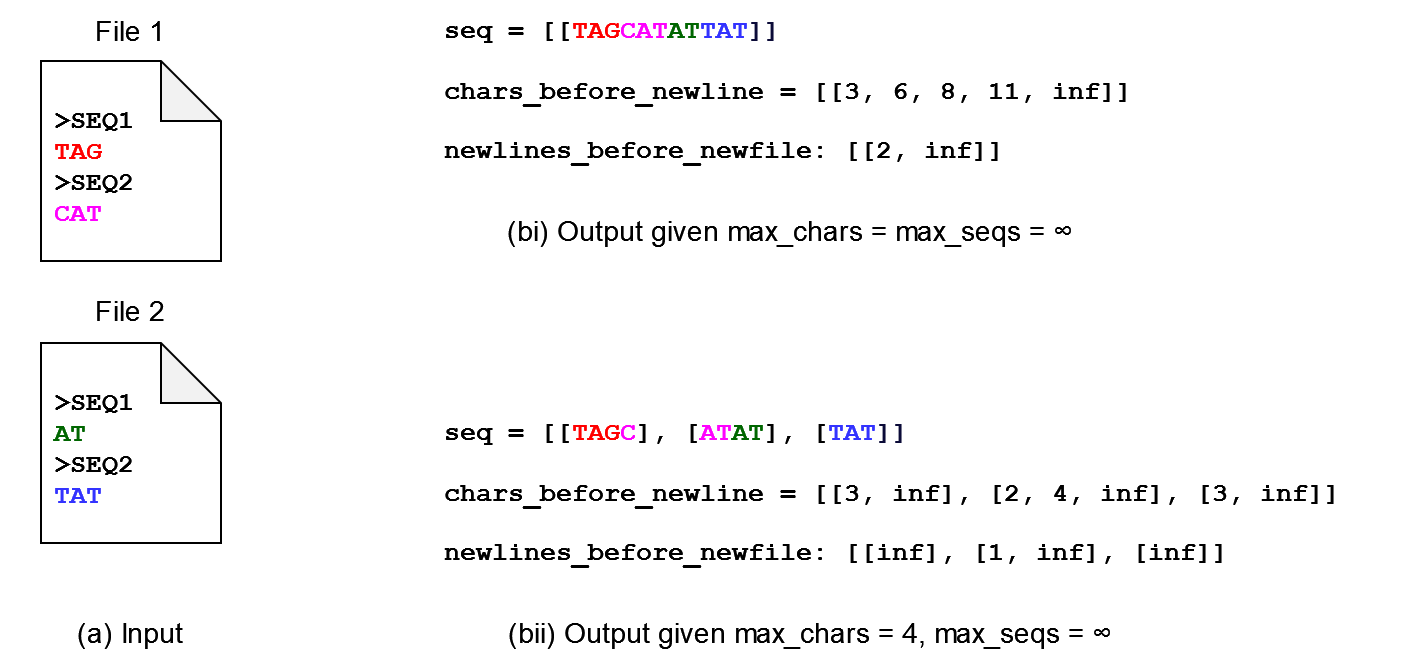
\includegraphics[width=\textwidth]{images/FastaqParser.png}
  \caption{(a) The input FASTA/FASTQ files with the sequences. (b) Outputs of the custom parser. In (bi) the entirety of the input in a single batch is read, whereas three batches are needed in (bii) since the maximum characters per batch is four. Sequences are color coded for easier interpretation.}\label{fig:FastaqParser}
\end{figure}

As a result of more logic involved with this parser, the performance is usually a bit slower than kseq++.
To test this, a FASTA file containing the human genome\footnote{\url{https://www.ncbi.nlm.nih.gov/projects/genome/guide/human/index.shtml}}\footnote{\url{https://ftp.ncbi.nlm.nih.gov/refseq/H_sapiens/annotation/GRCh38_latest/refseq_identifiers/GRCh38_latest_genomic.fna.gz}} and a FASTQ file from a study of early-life microbiota construction\footnote{\url{https://www.ebi.ac.uk/ena/browser/view/PRJEB32631}}\footnote{\url{ftp://ftp.sra.ebi.ac.uk/vol1/fastq/ERR340/004/ERR3404624/ERR3404624_1.fastq.gz}}~\cite{ecoli_genomes_3} were used.
The results and sizes of the files are shown in Table~\ref{tab:KlibVsReklib} and show that kseq++ is usually faster, especially for unzipped FASTA files.
These results were run on the Mahti supercomputer, whose specifications are discussed in Chapter~\ref{ch:Results}.
For decompression, zlib\footnote{\url{https://github.com/madler/zlib}} is used, the same as kseq++.
However, when parsing FASTQ, kseqpp\_REad is very comparable and since most of what the algorithm will be parsing are FASTQ files, as this use case deals with reads and not genomes, the performance drop is acceptable.
One disadvantage of kseqpp\_REad is that the title and quality string information are lost, so it cannot be applied to all workflows.

\begin{table}[]
\centering
\caption{Benchmarking results of kseq++ vs kseq++\_REad when parsing FASTA and FASTQ files in both zipped and unzipped formats. These values are averaged over 5 runs.}\label{tab:KlibVsReklib}
\resizebox{\textwidth}{!}{%
  \begin{tabular}{@{}lllll@{}}
  \toprule
                          & FASTA (2.2 GB)        & FASTA-zipped (928 MB) & FASTQ (3.1 GB)   & FASTQ-zipped (928 MB) \\ \midrule
  kseq++ time             & 2.2s                  & 13.5s                 & 3.7s             & 15.3s    \\
  kseq++ throughput       & 1024 MB/s             & 68 MB/s               & 838 MB/s         & 61 MB/s    \\
  kseq++\_REad time       & 4.2s                  & 15.2s                 & 4.1s             & 15.7s    \\
  kseq++\_REad throughput & 523 MB/s              & 61 MB/s               & 756 MB/s         & 59 MB/s    \\ \bottomrule
  \end{tabular}
}
\end{table}

\subsection{Preprocessing}

There are 2 steps for preprocessing the dataset.
The first is to bitpack it.
This means that the algorithm scans through the sequence produced by the previous step and converts $A$s to 0s, $C$s to 1s, $G$s to 2s and $T$s to 3s.
In binary, these can be represented with just 2-bit per character.
Thus, a u64 vector is created and the characters are packed in this vector in their original order.
This pass can be done in parallel, such that each thread processes the same amount of characters rounded to the nearest index which is a multiple of 64.
For example, given 200 characters, and 2 threads, thread 0 would process characters from 0 to 128, while thread 1 would process the rest.
In this small example, the ratio between the work done by the two threads is significant, as one thread does almost twice as much: $128 / (200 - 72) = 1.78$.
However, given that the number of characters in this case is in the order of millions or billions, one can say that each thread does the same amount of work.

During the same pass as bit-packing, another boolean vector of invalid characters is filled.
An invalid character is one which is not in the alphabet $ACGT$.
At the start, this vector is filled with 0s.
When an invalid character is seen in the sequence at an index $i$, the value of the invalid characters vector at index $i$ is set to 1.
Since this work is done in the same pass as bit-packing, it is also done in parallel, with the bitvector reserved beforehand.
Rather than a vector of booleans, in the implementation a vector of characters is used, as it was found to be faster.
When an invalid character is found, it is represented as if it were an A when it is bit packed, that is, as $00$.

The last preprocessing step is building the positions vector.
As discussed before, if a sequence has $C$ characters, then it has $C - k + 1$ $k$-mers.
The positions are thus u64s which represent the indexes in this sequence where a $k$-mer starts, and the next k characters, that index included, will be considered as a $k$-mer.
To do this position building, the chars\_before\_newline created in the parsing phase are used.
The positions can be generated with a single pass over this vector.
Figure~\ref{fig:Preprocessing1} shows an example of the preprocessing outputs discussed in this subsection.

\begin{figure}[t]
  \centering
  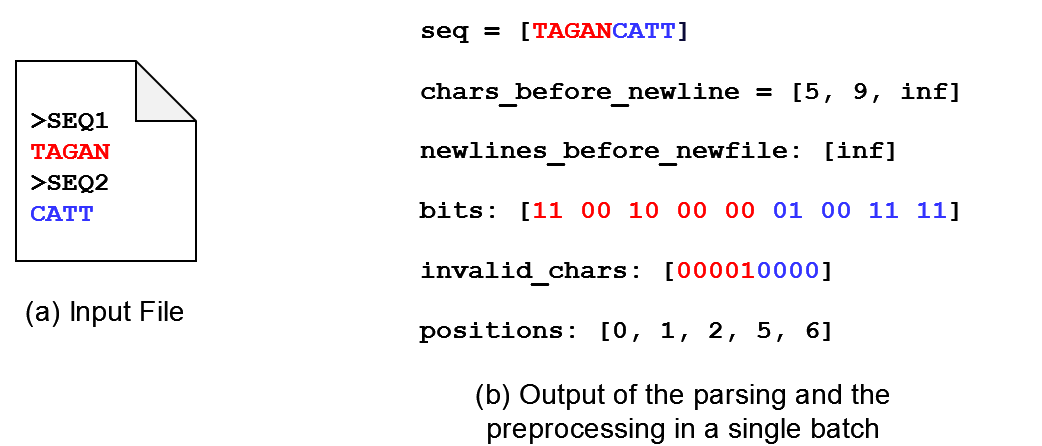
\includegraphics[width=0.8\textwidth]{images/Preprocessing1.png}
  \caption{An example of parsing and preprocessing in a single batch with the maximum characters per batch being $\infty$} \label{fig:Preprocessing1}
\end{figure}

The algorithm uses batching, so that each batch can only have a maximum number of characters and a maximum number of new sequences, whichever is reached first.
Since batching is being used, trouble would ensue if batching breaks a sequence in half, since characters may be shared between $k$-mers.
Hence the final $k-1$ characters must be copied from the previous batch to the start of the new batch in order not to miss any $k$-mers.
The amount may be less than this, as there is only a need for copying if the batching breaks the $k$-mers.
Figure~\ref{fig:Preprocessing2} shows an example where one needs to copy, and a case where copying is unnecessary.
There are also middle cases where one may need to copy some characters but less than $k-1$ characters.
This happens when the batching cuts off a sequence at its beginning, that is, before k characters have been parsed from it.
Copying is done in the parsing step, the first step discussed, so the rest of the components are oblivious to this step.

\begin{figure}[t]
  \centering
  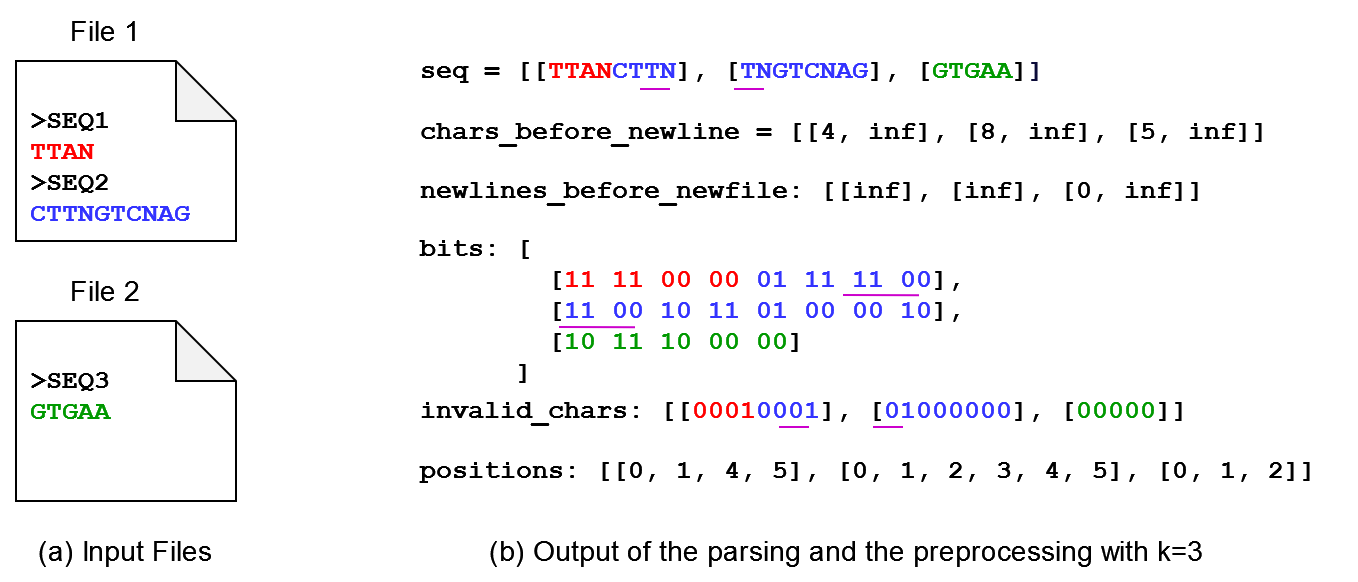
\includegraphics[width=\textwidth]{images/Preprocessing2.png}
  \caption{A second example of preprocessing, with the maximum characters per batch being 8. Notice how the string gets broken between the first and second batch, but not between the second and third. Overlapping areas have been marked with purple lines.}\label{fig:Preprocessing2}
\end{figure}

\subsection{Searching}

The index searching algorithm was discussed in Section~\ref{sec:SBWTQuerying}.
The only difference now is that the processing is done on the GPU.
Remember that the SBWT, the Poppys and the key-$k$-mer marks are already copied to the GPU.
Now the bit-packed sequence and the positions also need to be copied there.
Thus, each thread on the GPU handles a single position, since there is no relation between one $k$-mer search and the next.
As an optimisation, to save memory, and perform less memory accesses, one can overwrite the u64s of the positions with the u64s of the search result.
After this, the results can be copied back to memory and written to disk.
This GPU search function was created previously~\cite{Harri} but is now refactored and used in the new solution.
One change that this thesis has made to the previous implementation is to make it possible to query for $k > 32$ by always querying global GPU memory for the next two bits, rather than first storing the entire $k$-mer into a u64 and then querying that.
Although the performance difference between the previous and new kernel was not measured in isolation, this change was not shown to impact the overall performance of the algorithm from start to finish, since the kernel is only a small part of the bigger picture.

One more optimisation to searching which was used in previous works is presearching \cite{Presearch, SBWT, Harri}.
This is done right after loading the SBWT to the GPU, however, it was chosen to discuss it now in order not to confuse the reader with too much disjoint information at the beginning.
The notion behind presearching is that one can search for the first part of the $k$-mers beforehand, store these in memory, so then rather than recomputing these, they can be loaded from memory and continue the search continues from there.
To do this presearching, the left and right pointers are moved forward by a certain amount $k_p$ for every permutation of a $k_p$-mer.
Thus, given for example $k_p=2$, the combinations are: $AA, AC, AG, AT, CA, CC, \ldots, TG, TT$.
Represented as binary, they become: $0000, 0001, 0010, 0011, 0100, 0101, \ldots, 1110, 1111$.
The decimal representation is then: $0, 1, 2, 3, 4, \ldots, 14, 15$.
Thus note that these can be used as the indexes to both store and later retrieve the presearched left and right pointers for $k_p$.

In the example, 16 memory spaces are needed.
More generally, $4^{k_p}$ are needed for each of the left and right pointers, where each memory space contains a u64.
Thus, the final formula for the total number of bits to store the presearch results is \[4^{k_p} \times 64 \times 2 \quad \mathit{bits}.\]
Ideally, one would presearch with $k_p = k$, however, the memory requirements for this would be massive, as the formula is exponential on $k_p$.
If $k_p=k=31$, this would require $4^{31} * 64 * 2 / 8 / 1024 ^ 3 \approx 9$ billion GB.
As a result, similar to the previous GPU method~\cite{Harri}, $k_p=12$ is used.
With this, 250MB of data are needed in total for the presearch data.
Algorithm~\ref{alg:SearchWithPresearch} shows the final search algorithm.

\begin{algorithm}
	\KwIn{\newline
    A sequence $S = c_1, c_2, \ldots, c_k$ \newline
    Bitvectors $b_A, b_C, b_G, b_T$
    c-map $C$
    Presearch size $k_p$
    Presearch maps $presearch_{\mathit{left}}$ and $presearch_{right}$
	}
  $\mathit{left}$ = $presearch_{\mathit{left}}[c_1, \ldots, c_{k_p}]$

  $\mathit{right}$ = $\mathit{presearch}_{right}[c_1, \ldots, c_{k_p}]$

  \ForEach{c \textbf{in} S[($c_{k_p} + 1$) \ldots k]}{
    $\mathit{left}$ = $C[c]$ + rank ($b_c$, $left$)

    $\mathit{right}$ = $C[c]$ + rank ($b_c$, $right + 1$) \-- 1

    \If{$\mathit{left}$ > $\mathit{right}$} {\
      \textbf{return} not found
    }
  }

  \textbf{return} $left$

  \caption{Index Search function with presearch.}\label{alg:SearchWithPresearch}
\end{algorithm}

\subsection{Results Printing}

For results printing, there are three output formats, but programmatically they follow the same interface.
This means that in general, they all print to a memory buffer first and then these buffers are printed to disk.
Printing to buffers is done in parallel, meaning that each thread has an equal amount of indexes to print and each thread prints to its own equally sized buffer, and then the buffers are printed to disk sequentially.
The reason it was opted to parallelise this pass, rather than simply printing to disk, is because of the conversions which need to be done, from the binary representation in memory, to the representation on disk.
For this step, the search results are used, the chars\_before\_newline to know where to split each sequence, the seqs\_before\_newfile to know when the algorithm needs to open the next file, and the invalid characters list to differentiate these from the characters which were not found.
The feature to differentiate invalid characters from the not-founds is not found in Themisto or its precursors, and is hence another new contribution.

Next, each output format is discussed.
Figure~\ref{fig:IndexResultsPrinting} serves as a good visualisation of how the characters are written to disk.
It is important to note that the only implementation difference between these formats is how they print each value.
The available values which they can print are the following: a found index, a not-found index, an invalid character, or a newline.
The first to consider is the ASCII format, where the indexes are printed as a space-separated list of values.
The values for the indexes are simply u64s, so they can be printed as their ASCII counterparts.
The not-found values are represented as $-1$, invalid characters as $-2$, and newline values as the expected line feed character \textit{\textbackslash n}.
This format was the one that saw the largest benefit from parallelisation, as the operation to convert from binary to ASCII, especially for larger numbers, takes significant CPU time, due to the need of performing many division and modulus operations which are computationally expensive.
In order to convert from binary to ASCII, the algorithm created by James Anhalt\footnote{\url{https://github.com/jeaiii/itoa}} is used.
This was benchmarked on a dummy dataset internally against the \textit{to\_string} algorithm from the GCC C++ standard library and against the \textit{format\_decimal} algorithm by \textit{fmt}\footnote{\url{https://github.com/fmtlib/fmt}} library and it was found that the algorithm by Anhalt was significantly faster than these alternatives.
It is also the fastest algorithm in other benchmarks\footnote{\url{https://jeaiii.github.io/itoa/}}.
No detail will be given as to how the u64 to ASCII algorithm works and what differentiates it from other algorithms, as this problem is a deep rabbit hole and could make for its own thesis.

\begin{figure}[t]
  \centering
  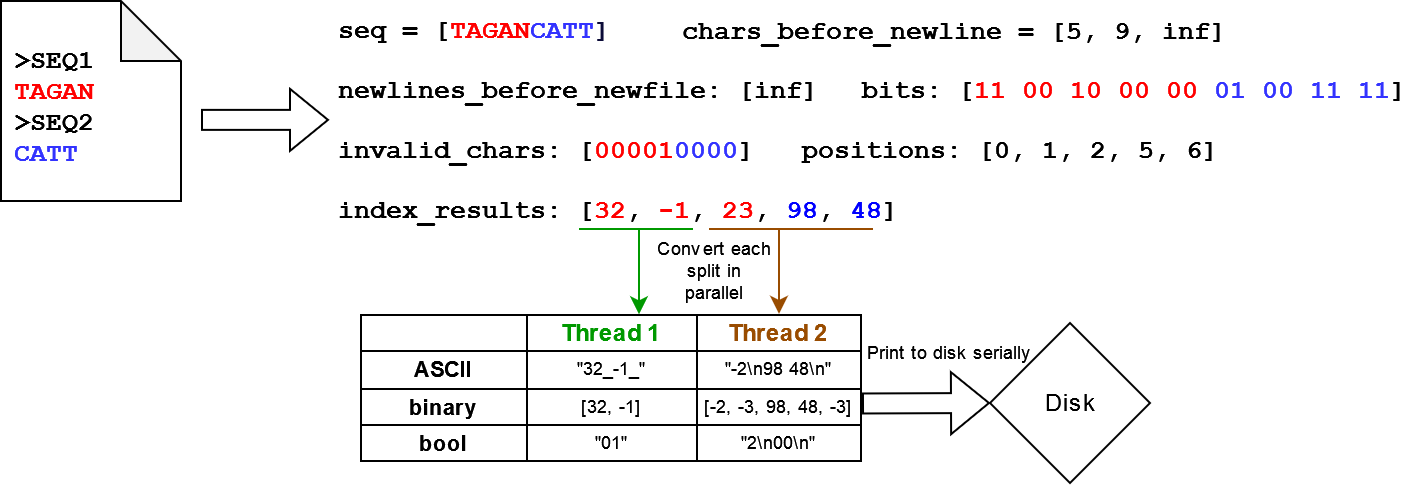
\includegraphics[width=\textwidth]{images/IndexResultsPrinting.png}
  \caption{The results printing pipeline from FASTA/FASTQ files to printing to disk in a single batch. The parallelisation of this is also visualised. For the ASCII and bool formats, these use usual 8-bit ASCII characters for their representation, whereas for the binary format uses a contiguous array of u64s.}\label{fig:IndexResultsPrinting}
\end{figure}

The second format is the binary format.
In this format, each element that is printed takes 8 bytes, as everything is printed as a u64.
Results are printed as they are.
Meanwhile, not-found values are printed as the maximum u64 value, that is, $2^{64}$, invalid values are printed as $2^{64} - 1$, and newlines are printed as the $2^{64} - 2$.
In C++, unsigned integers loop back when they overflow, so that one can say that the values for not-founds, invalids and newlines are $-1$, $-2$, and $-3$ respectively.
This method would be faster and with less memory requirements than the ASCII format if most of the indexes contain more than 8 bytes.
The ASCII format requires at most 20 bits for each character, since the maximum value of u64 is 20 characters long, plus another character for the whitespace character which separates the values.
However, as will be seen in Chapter~\ref{ch:Results}, while not drastically slower than the ASCII format, this method ends up taking a lot more space, since the indexes are usually not too large.

The last format is dubbed the boolean format.
In this format, the sequences are separated with newlines, as in the ASCII format.
However, for the values, a single byte is used.
For the found values, the ASCII character for 0 is printed, then the not-founds are represented with a 1 and the invalids are represented with a 2.
This makes it the smallest format and also also the fastest to print, at the cost of losing the index information, that is, where the $k$-mer is found within the SBWT.
As a result, it is not suitable for the second phase, since the indexes are needed.
However, it is the best format for users who simply want to know if the $k$-mers of their sample exist within the SBWT or not.

\section{Phase 2:  Color Search}

Now the color searching phase will be described.
A small summary is the following: (a) Load the color data structure from disk into the GPU, (b) parse the indexes output of phase 1 from disk and put them in the GPU, (c) search for the color set associated with each index within the GPU, (d) combine all the colors of a sequence together in the GPU, (e) copy the results back from GPU into main memory and write the color sets for each sequence to disk.
Each of these steps, how they are parallelised, and what data structures they produce will be elaborated on in the next section.
Similarly to the index search, the data structures introduced in this section are summarised and explained in a different manner to aid understanding, in Appendix~\ref{app:ColorSearchDataStructures}.

\subsection{Preliminaries and Definitions}

Before discussing the implementations, some mechanisms of how work is done in the GPU need to be introduced.
A unit of work on the GPU is done with a \textit{warp} (or \textit{wave} in AMD terminology).
Each warp in an NVIDIA GPU consists of 32 threads, and 64 in an AMD GPU.
This means that threads within a warp execute at the exact same time under normal conditions.
Threads in a warp can also communicate with one another by sharing the contents of their variables, using what are known as shuffle operations\footnote{\url{https://people.maths.ox.ac.uk/gilesm/cuda/lecs/lec4.pdf}}\footnote{\url{https://docs.nvidia.com/cuda/cuda-c-programming-guide/index.html#warp-shuffle-functions}}\footnote{\url{https://developer.nvidia.com/blog/using-cuda-warp-level-primitives/}}.
For example, if each thread has a variable $X$, this can be broadcasted to all the threads in the same warp.
One common use case of this feature is to get the sum of the variable across the warp.
Another approach is shared memory\footnote{\url{https://docs.nvidia.com/cuda/cuda-c-programming-guide/index.html#shared-memory-variable-declarations}}, which works on the block level.
However, neither shared memory nor blocks will be discussed since they are irrelevant to the rest of the thesis.

A point to remember from Section \ref{sec:Pseudoalignment} is that all $k$-mers in the SBWT are colored, except for dummy $k$-mers.
This means that if a $k$-mer is found in the SBWT, it is colored, and if not, then it is blank.
In this thesis, a colored sequence means refers to sequences that have at least one found $k$-mer, otherwise the sequence will be a \textit{blank sequence}.

\subsection{Loading the Colors}

Now starts the implementation part of this section, with the description of how the colors are loaded.
This data structure is created by Themisto, and needs to be loaded from disk.
The data structure itself is described in Section~\ref{sec:Pseudoalignment}, and all that is added is that the Poppy data structures need to be built for the $\mathit{is\_key\_k\_mer}$ and $\mathit{is\_dense\_marks}$.
This data structure also contains some additional variables such as the number of colors $\mathit{num\_colors}$.
The process is done entirely serially as the items are loaded from the file and the Poppy of the bit-vectors is created serially as well.
These components are then all loaded into GPU memory and kept there until the end.

\subsection{Loading the Indexes}\label{subs:IndexesLoading}

Now the indexes are loaded from disk as they were printed in phase 1.
For this subsection, Figure~\ref{fig:IndexesLoading} shows the final product.
For each sequence the count is taken of how many indexes were found, not found, or are invalid.
Similarly to the first phase, a vector is also created, called the $\mathit{seqs\_before\_newfile}$, which stores a cumulative sum that indicates at which point the algorithm needs to stop considering sequences to be from one file and start considering them as originating from the next file.
A new count is started at the very beginning of a batch or whenever a newline symbol is seen, these symbols being the line feed character '\textbackslash n' for ASCII and a -3 for the binary format.
Again, the boolean format is not suitable for pseudoalignment and cannot be used for phase 2 since this method does not have the indexes.
Similar to reading in phase 1, batching is used with a set maximum number of characters and maximum number of sequences per batch.

For parsing, no special techniques are used.
Characters are read one by one, and for the ASCII format, the na\"ive method of reading one digit and adding it to the previous value multiplied by 10 is used.
This is faster than the C++ standard library, as the standard library implementations usually have some form of error checking involved.
For the binary format, the algorithm simply reads 64 bits at a time.

\begin{figure}[t]
  \centering
  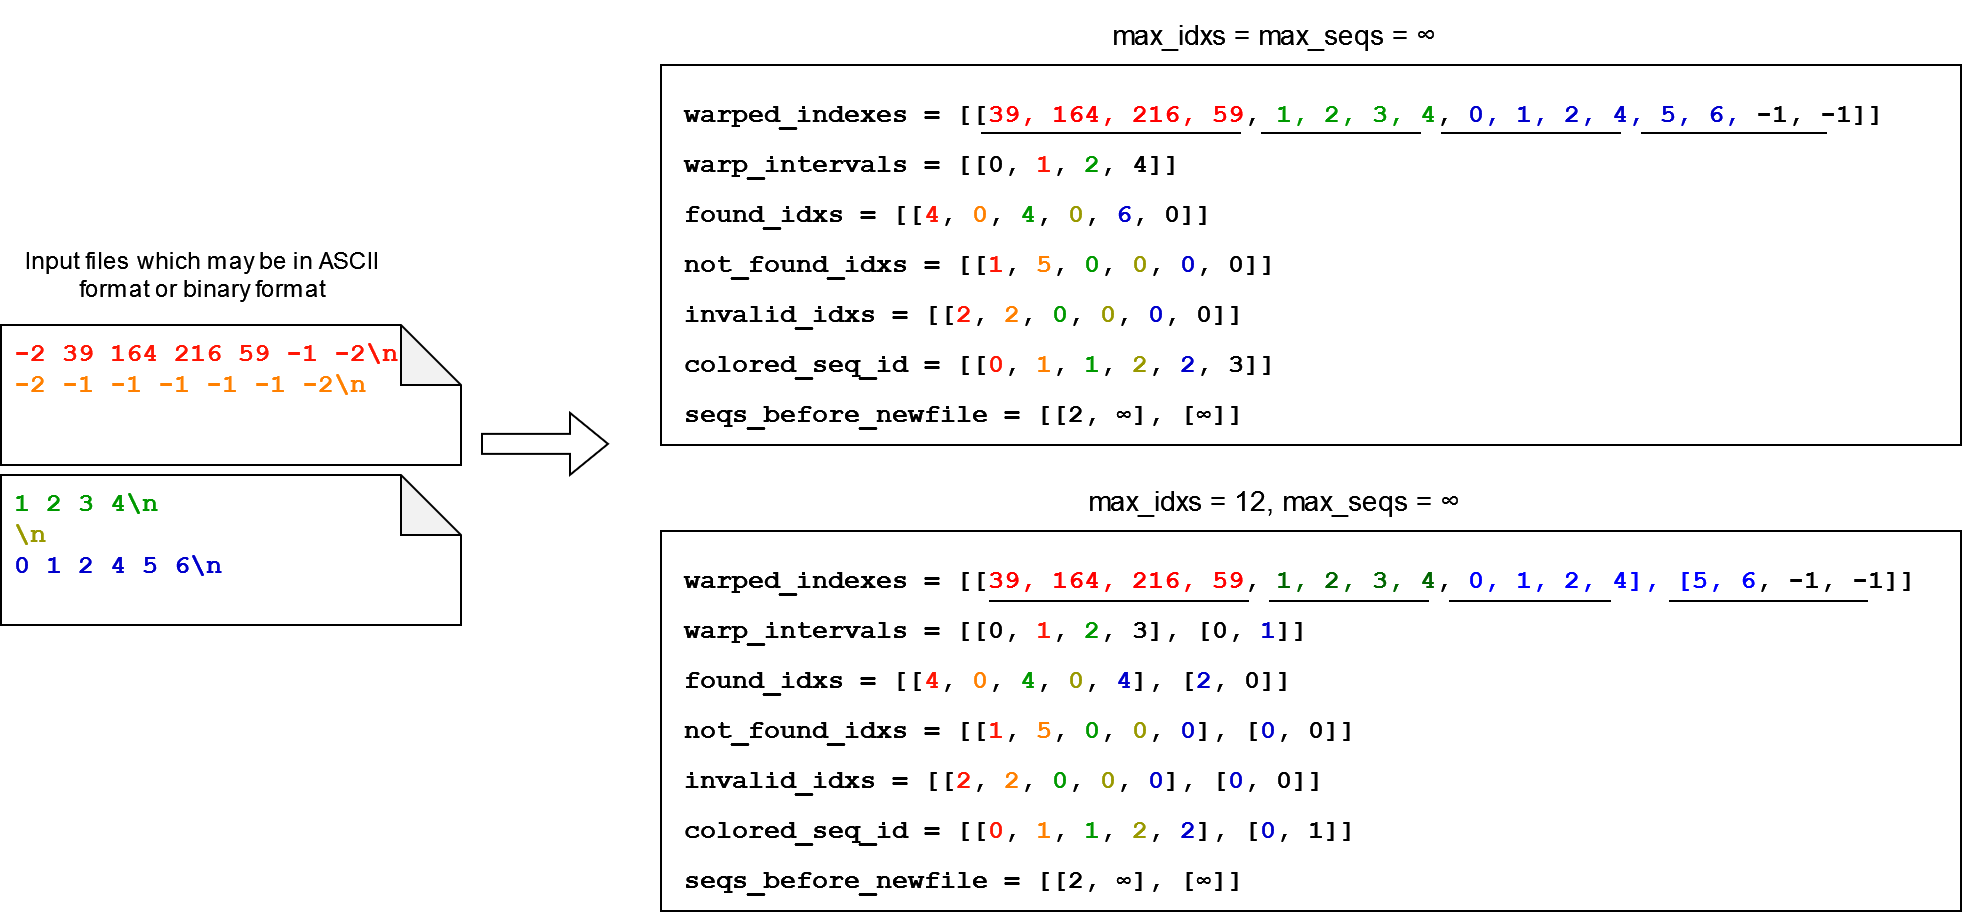
\includegraphics[width=\textwidth]{images/IndexesLoading.png}
  \caption{Example of loading from an ASCII or binary index files and populating the necessary data structures with two different configurations, one where the maximum characters per batch is infinite and one where it is limited to 12, such that the last sequence is broken in two. Note that the last values of the $\mathit{found\_idx}$, $\mathit{not\_found\_idx}$, $\mathit{invalid\_idx}$ and, $\mathit{colored\_seq\_id}$ are because the algorithm needs to consider the next sequence to come.}\label{fig:IndexesLoading}
\end{figure}

Indexes that are not found or invalid are not stored.
This makes the algorithm a lot more efficient, both in terms of time and memory.
The respective counters for the sequence that these indexes belong to are increased, but they are not stored as part of the index list.
Thus, blank sequences effectively take no space, besides the small variables for their counters.
Meanwhile, the indexes of colored sequences are stored contiguously, but between one sequence and the next, padding is used up to the next multiple of the warp size.
This technique and the reasoning for it will be made clearer in Subsection~\ref{subs:ColorSearch}.

Since a sequence may be larger than the warp size, these $\mathit{warped\_indexes}$, as they are called, are then separated via another list called the $\mathit{warp\_intervals}$.
The first entry of this list is always 0, and another entry is added whenever a new sequence causes more $\mathit{warped\_indexes}$ to be added which belong to a new sequence.
Whenever that happens, the new entry which is added will be the cumulative sum of how many warps the algorithm has until the end of that sequence.

Besides the aforementioned variables, another list exists and is called the $\mathit{colored\_seq\_id}$.
This stores an unsigned integer for every sequence, and it indicates which number colored sequence this sequence is.
If a sequence is blank, a $\mathit{colored\_seq\_id}$ is still stored for it, and for convenience, the previous in the list is copied for it, but it might as well be padding as it is later ignored.
This list is then is used in Subsection~\ref{subs:ColorsPrinting}.

\subsection{Searching}\label{subs:ColorSearch}

The next part is the color searching, which is entirely done on the GPU but is split into two kernel calls: Searching and Post Processing.
First, the indexes are copied to the GPU and memory is reserved for the color results.
Note that since blank sequences do not produce any indexes, they also do not use any computations on the GPU later on, thus the algorithm runtime depends on the number of warps spanned by the colored sequences.
Next, the values reserved for the color results are set to 0 using \textit{memset}.
Each thread handles a single index and searches for its color set type, which is sparse or dense, its start index, and its end index, using the same method as Algorithm~\ref{alg:ColorSearch}.
If a thread has a padding index, then it exits immediately.
To do this, a separate GPU functions gets booleans from bitvectors and another extracts a normal u64 from the compact vectors.
The result of this step are the indexes where the color sets start and end within their respective dense or sparse arrays.

The next step of the kernel is to extract and combine the color sets.
First, a small optimisation is performed, which is to get the minimum and maximum color id which exists within the color set of each thread.
To get the minimum present color of a dense color set, the algorithm iterates through the bitvector from the starting point of the color set until the first set bit is found.
Then, to get its maximum, it can simply negate the end index of this color set with the starting index, both of which were found before.
On the other hand, to get these values for sparse colors, one needs to access the sparse color set array and obtain the ones at the start and end indexes to get the minimum and maximum present color id respectively.
Next, an XOR shuffle is performed to broadcast these two values to the other threads inside the warp, so that each thread knows the minimum and maximum color if of all threads within the warp.
To broadcast a value using shuffle, the algorithm needs to perform $log_2(warp\_size)$ steps, as is visualised in Figure~\ref{fig:ShuffleXor}.
Two shuffles need to be performed: one for the minimum and another to broadcast the maximum.
Due to the padding technique when reading the indexes, all threads in each individual warp only contain indexes belonging to a single unique sequence, that is, a warp will not mix colors of different sequences together.

\begin{figure}[t]
  \centering
  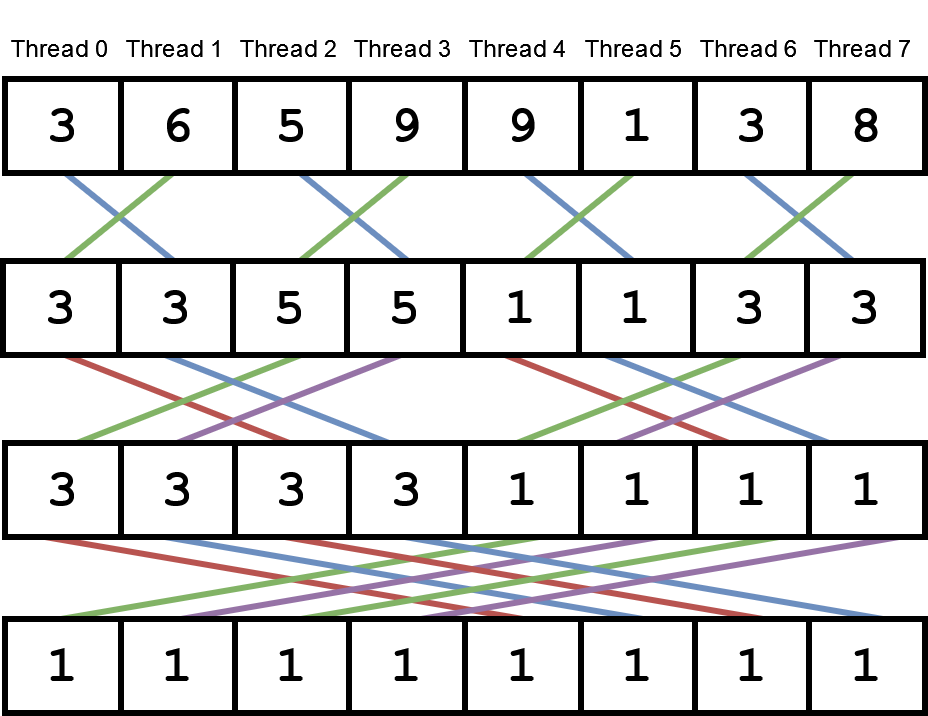
\includegraphics[width=0.7\textwidth]{images/ShuffleXor.png}
  \caption{An example of how data is shared between threads at each step of an XOR shuffle operation to find the min value of the warp. The warp size for this visualisation is 8, hence there are $log_2(8) = 3$ shuffle operations.}\label{fig:ShuffleXor}
\end{figure}

The next step is to iterate through all the colors in the color sets from the minimum and maximum of the warp, and set a boolean value to whether the color exists in the color set of that thread or not.
To get the color presence in the dense array, one can simply do a boolean access in the bitvector at the index of the color.
When it comes to the sparse array, one then needs to go through the array and check if the current color id matches the value in the array.
Luckily the sparse arrays are sorted so the algorithm can do this check in a single step, without going through the whole array for every query, thus going through the whole array only once, as the color presence of every color is checked.

After the color presence of a color is obtained, $\mathit{ballot()}$ is called, where an unsigned integer is created which has as many bits as the warp size, and each thread in the warp sets its respective bit in this integer to 1 if the color is present, and 0 otherwise.
The result of this ballot is broadcasted to all threads in the warp, but it is thread 0 that performs a popcount on this result and stores the color count to device memory.
Notice that this result is at most 32 in the case of NVIDIA devices, and 64 in the case of AMD devices.
This means that a 32-bit integer representation is used for the NVIDIA case, and a 64-bit integer is used for AMD devices.
Furthermore, it also means that the popcount of each of these color counts can be stored in an 8-bit unsigned integer, which is why a list of u8s is used to store these intermediate results, in order to save memory space and thus be able to process more indexes per batch.
The $\mathit{ballot()}$ function is visualised in Figure~\ref{fig:Ballot}, whereas the pseudo code until this point of the color search is found in Algorithm~\ref{alg:GpuColorSearch}.

\begin{figure}[t]
  \centering
  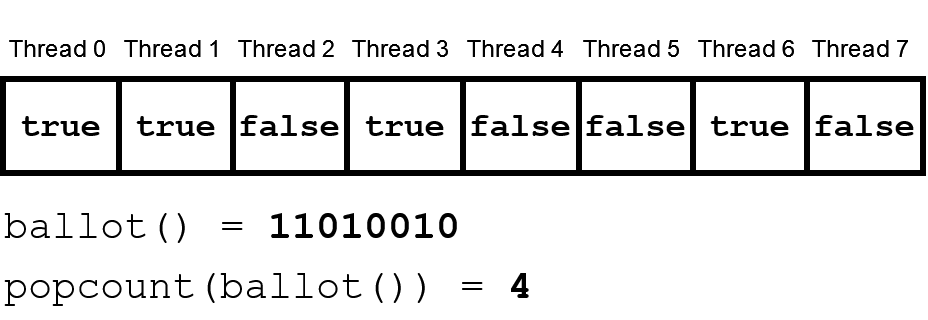
\includegraphics[width=0.7\textwidth]{images/Ballot.png}
  \caption{An example of a ballot operation for a warp of size 8. The ballot operation is called only once in each of the threads, whereas the popcount function on the result of this operation needs to be called by thread 0 only, since this is the one which will be storing the result in this case.}\label{fig:Ballot}
\end{figure}

\begin{algorithm}
	\KwIn{ \\

    $\mathit{warped\_indexes}$

    $\mathit{warp\_size}$

    $\mathit{num\_colors}$

    $\mathit{dense\_arrays}$

    $\mathit{sparse\_arrays}$
	}

  $\mathit{thread\_idx}$ = GPU thread id

  $i$ = $\mathit{warped\_indexes[thread\_idx]}$

  Get $\mathit{start}$, $\mathit{end}$ and $\mathit{is\_dense}$ using $i$ as an input to Algorithm~\ref{alg:ColorSearch}.

  \If{$\mathit{is\_dense}$} {\newline

    $\mathit{min\_id}$ = Traverse $\mathit{dense\_arrays}$ from $\mathit{start}$ to get first set bit

    $\mathit{min\_non\_zero\_color}$ = $\mathit{start}$ - $\mathit{min\_id}$

    $\mathit{max\_non\_zero\_color}$ = $\mathit{end}$ - $\mathit{start}$

  }\Else{ \\

    $\mathit{min\_non\_zero\_color}$ = $\mathit{sparse\_arrays[start]}$

    $\mathit{max\_non\_zero\_color}$ = $\mathit{sparse\_arrays[end - 1]}$
  }

  $\mathit{min\_non\_zero\_color}$ = xor\_shfl($\mathit{min\_non\_zero\_color}$)

  $\mathit{max\_non\_zero\_color}$ = xor\_shfl($\mathit{max\_non\_zero\_color}$)

  $\mathit{array\_idx}$ = $\mathit{start}$

  \ForEach{$\mathit{color\_id}$ \textbf{in} [$\mathit{min\_non\_zero\_color}$ \ldots $\mathit{max\_non\_zero\_color}$]}{

    \If{$\mathit{is\_dense}$} {\newline

      $\mathit{color\_present}$ = ($\mathit{dense\_arrays[array\_idx]}$ = 1)

      ++$\mathit{array\_idx}$

    }\Else{\newline

      $\mathit{color\_present}$ = ($\mathit{sparse\_arrays[array\_idx]}$ = $\mathit{color\_id}$)

      \If{$\mathit{color\_present}$} {\newline

        ++$\mathit{array\_idx}$
      }
    }

    $b$ = ballot($\mathit{color\_present}$)

    \If{$\mathit{thread\_idx}$ \% $\mathit{warp\_size}$ = 0} {\newline
      $\mathit{results}$[$\mathit{num\_colors}$ * $\mathit{thread\_idx}$ / $\mathit{warp\_size}$ + $\mathit{color\_idx}$] = pop\_count($b$)
    }

  }

  \caption{GPU Color Search}\label{alg:GpuColorSearch}
\end{algorithm}

The result of this step is a color count for each color for each warp, where many warps may belong to the same sequence.
Thus, the last step is to postprocess the results by combining the results of the same sequence into a single list.
First, memory is reserved for these u64 results and the warp intervals created in Subsection~\ref{subs:IndexesLoading}, the latter of which can now be copied to the GPU.
Both of these two arrays use the same memory space previously used by the indexes, to maximise memory usage.
Now, one thread is created for every color in every sequence.
Each thread gets a cumulative sum of a single color in the whole sequence and then stores this sum in the new u64s.
These final results can then be copied to CPU memory, as they are now ready for printing.
A visualisation for the post processing step is in Figure~\ref{fig:PostProcessing}.
The disadvantage of this postprocessing method is that if the number of indexes in the colored sequences varies by a lot, then the sequences would produce a disproportionate number of color sets, meaning that some threads would need to do more work.
Luckily, the ballot step of the first phase reduces the work done in this step and the memory required by a factor of 32 on NVIDIA devices and a factor of 64 on AMD devices.
These two factors, that is, both the work done and memory used, is also the reason why it was opted to only put and process colored sequences in the GPU.
Also notice that some threads will only need to only expand the value of the color id from u8 to u64 and store it into the new results, without doing any additions.
Moreover, a flaw of this design is that, given sparse color sets, that is, most colors result in a count of zero, then this design ends up wasting a lot of space, as these zero counts still need to be allocated and also copied back to CPU memory.

\begin{figure}[t]
  \centering
  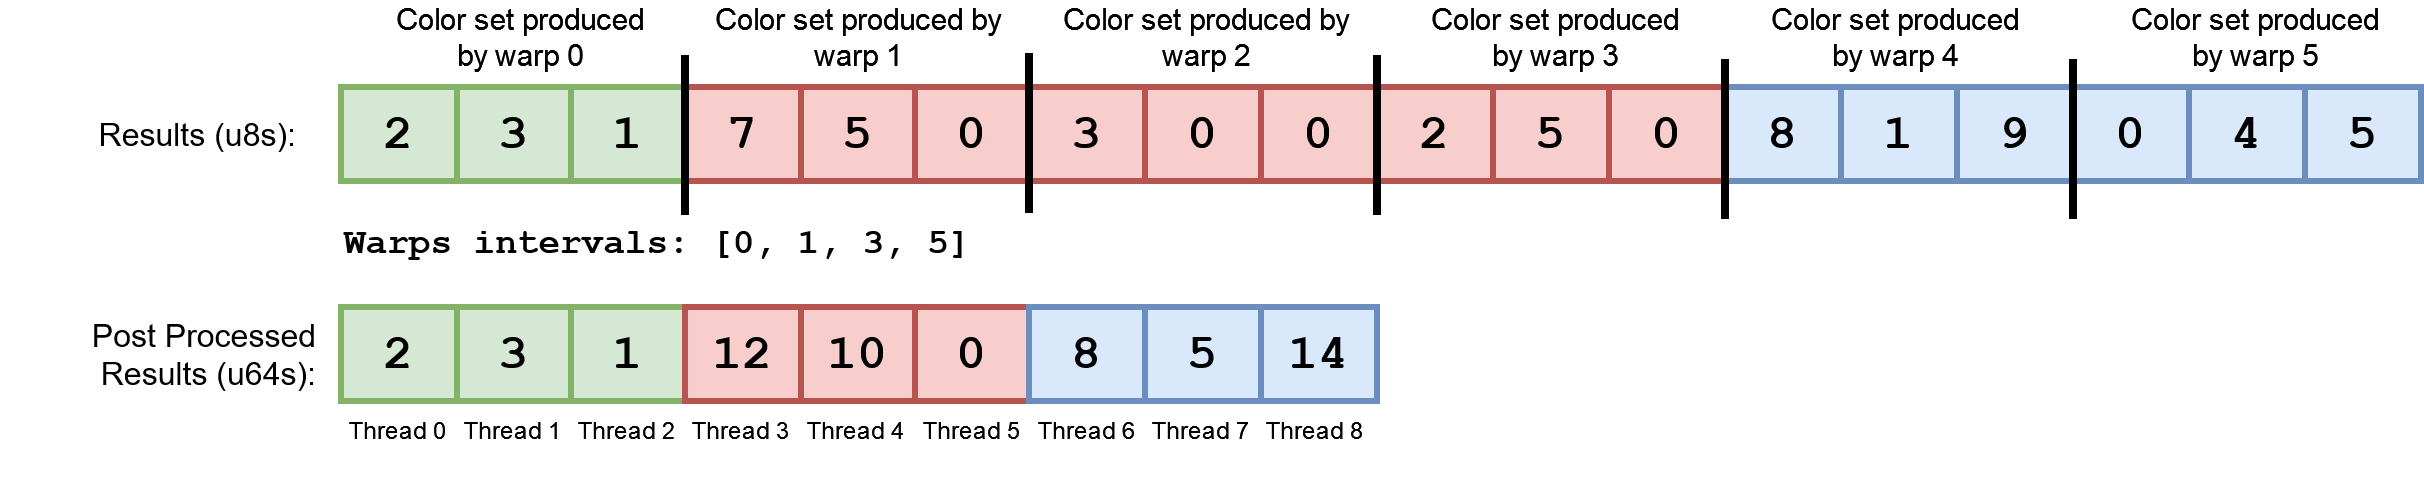
\includegraphics[width=\textwidth]{images/PostProcessing.png}
  \caption{A visualisation of the post processing done on the colors. Each thread handles a single color from each sequence. As a result, some threads may end up doing more work than others if a different number of $k$-mers are found from each sequence. In this case, the middle sequence had more $k$-mers found, which meant that it produced more color sets: 3 warps worth of color sets. Hence, the post processing step does 3 sums for this sequence.}\label{fig:PostProcessing}
\end{figure}

\subsection{Results Printing}\label{subs:ColorsPrinting}

The final step of this last phase is to print the results.
In order to print, besides the colors themselves, the counts for the found, not-found and invalid indexes are provided, alongside the $\mathit{coloured\_seq\_id}$ and the $\mathit{seqs\_before\_newfile}$.
Similarly to the results printing in the first phase, the results are first printed to buffers in parallel and are then printed to disk serially.
For this phase, there are also three output formats: ASCII, binary, and CSV.
In the ASCII format, the colors are printed as space-separated values, where the color id is printed if it appears in the sequence, and each sequence is put on its own line.
Similarly to the previous phase, the boolean format prints each color as a u64 sequentially, where the maximum u64 is used to represent a new line.
These two formats could be seen as the sparse representation outputs, and the CSV is the dense output.
The CSV format prints a comma separated 1 or 0 for each color, where 1 means that the color is present in that sequence and 0 means it is not.
Figure~\ref{fig:ColorsPrinting} shows an example of these three results formats.

When printing to buffers in parallel, each thread handles an equal number of sequences, whether colored or not.
This may lead to some threads doing more work, as colored sequences take much longer to process for the ASCII and binary formats, especially when the color set size is big.
Reads, however, are usually distributed randomly, so the threads should statistically do the same amount of work
Before printing, thresholding is also done in this part.
The contribution of this thesis to this space is the differentiation between thresholding invalid $k$-mers as well as $k$-mers which were not found, the latter of which was included in Themisto.
So the user can choose to ignore one of them, both, or none at all.
Another advantage over Themisto is that the results are always output in ascending order, whereas Themisto may shuffle the results within a single sequence.
Lastly, since a sequence may be split into two batches, the colors and other sequence properties of the last sequence of a batch are copied over to the first sequence of the next batch in order not to lose any information.

\begin{figure}[t]
  \centering
  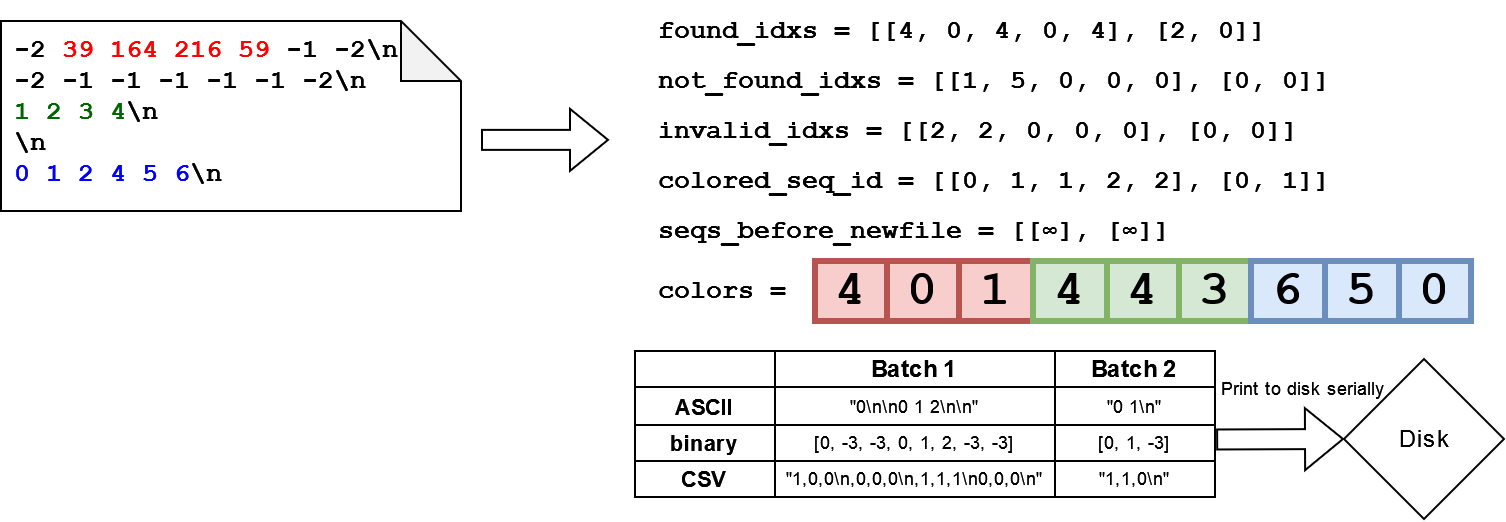
\includegraphics[width=\textwidth]{images/ColorsPrinting.png}
  \caption{A visualisation of the printing of the colors in all three formats. Here, $\tau=0.7$ is used, ignoring the kmers which are not found or invalid.}\label{fig:ColorsPrinting}
\end{figure}

\section{Other Optimisations and Parallelism}

In this section general optimisations used throughout the algorithm will be described.
These were not discussed during the general discussion of the two phases as they were not necessary to understand those topics, and they would have added a lot of complexity to an already complex topic.

\subsection{Curiously Recurring Template Pattern (CRTP)}

The first and simplest optimisation is the Curiously Recurring Template pattern which is popular for C++ development.
For those unfamiliar with C++, when a child class inherits a parent class and polymorphism takes place, a virtual table is created, which indicates the correct function to call to the program.
Thus, when a call to an inherited function is done, another call to the virtual table must be done, which is usually expensive as it requires another memory access.
CRTP allows programmers to do inheritance without the need for virtual tables, with the penalty being the use of templates, which make the code slightly less maintainable.
This optimisation was especially beneficial for the results printing, as some of the methods there are called billions of times, and traditional inheritance is still used in a lot of places where methods are not called as often.

\subsection{Multithreaded Pipeline}

In the two phases, there are some components that are dependent on one another, and others that are not.
Furthermore, since it is a pipeline, an earlier component can start processing the next batch while the later component is processing an earlier batch.
This is done by inheriting all producer components from a parent component called the \textit{SharedBatchesProducer}.
By using semaphores, it is ensured that all components can run in parallel, while still being able to share the memory of the buffers that the producers and consumers share safely.

\subsection{Pinned Memory}

For variables that need to be copied to and from the GPU, it is possible to use pinned memory on the main memory in order to speed up memory transfers.
To do this, all the programmer needs to do is to reserve the memory space beforehand using \textit{cudaMallocHost}\footnote{\url{https://docs.nvidia.com/cuda/cuda-runtime-api/group__CUDART__MEMORY.html}} or \textit{hipHostMalloc}\footnote{\url{https://rocm-developer-tools.github.io/HIP/group__Memory.html}} if using HIP.
Pinned memory can be copied to the GPU directly, whereas more care needs to be taken by pageable memory as this could be moved while copying is taking place, whereas pinned memory is guaranteed to remain in the same location within memory until it is freed\footnote{\url{https://developer.nvidia.com/blog/how-optimize-data-transfers-cuda-cc/}}.
This feature sped up transfers to and from GPU by almost twice, which is a significant difference for this use case as there are a lot of large transfers.
The drawback of reserving most of the memory beforehand is that large amounts of contiguous blocks need to be reserved at once.
This can be difficult to manage for the operating system, and in fact often contributes to a significant overhead at the start of the algorithm
Luckily this overhead is constant, so as the datasets get larger, this overhead becomes less and less significant, and for smaller datasets, a smaller memory can be reserved for the algorithm, which is a setting that can be altered by the user.
That said, for other variables which do not need to be communicated to or from the GPU, normal paged memory is used.

\subsection{Streams}

Often, larger datasets will be split into multiple files.
The code takes advantage of this by providing an algorithm that can take advantage of this, by being able to process multiple files at once.
This means that the pipeline is duplicated and the number of files can be split between each stream.
The term \textit{stream} is used to indicate each pipeline.
This means that, for example, given seven files and three streams, then stream 0 would handle three files, and streams 1 and 2 would handle two files each.
The two streams can then share the same SBWT or colors data structure in phases 1 and 2 respectively.

The benefit of using streams is that reading from disk and outputting to disk can also be done in parallel.
This is especially useful when using a multi-disk setup, or if the device in use can support this feature.
However, even if not using any of the above two hardware devices, two more advantages are universally applicable.
The first and more obvious is that by using streams, the CPU and disk can be kept more busy.
The second is the use of GPU streams.

Using a single stream with GPUs, the process is: (a) copy some data to the GPU, (b) do some processing, and (c) copy the data back to main memory.
By using multiple streams, each stream still does the same three steps, however, if multiple streams are used, the GPU can interleave the memory transfer of one stream with the processing of another\footnote{\url{https://developer.download.nvidia.com/CUDA/training/StreamsAndConcurrencyWebinar.pdf}}.
Memory transfers from GPU can also be interleaved with memory transfers to GPU on some devices.
Figure~\ref{fig:Streams} shows this visually.
The number of streams is configurable by the user, but is capped based on the number of files, so that the number of streams is always smaller or equal to the number of files that need to be processed.

\begin{figure}[t]
  \centering
  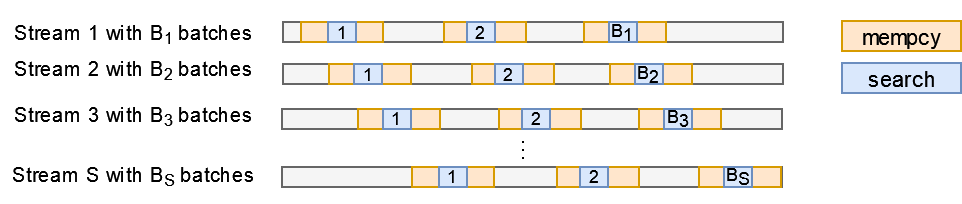
\includegraphics[width=0.8\textwidth]{images/Streams.png}
  \caption{A visualisation of using streams and their benefit on GPU processing, where memory transfers are interleaved with processing. The batch number is also displayed.}\label{fig:Streams}
\end{figure}

\subsubsection{Load Balancing}

An additional optimisation for streams is to load balance the streams.
Notice that if some files are large while others are very small, then different streams might have very different workloads.
Thus, the algorithm considers load to be based on file size.
As such, before assigning files to streams, they are analysed for their size and then a greedy algorithm called the Longest Processing Time first (LPT)~\cite{LPT1, LPT2}.
Here, an array is created for each stream, the file sizes are sorted such that the largest file is always chosen first and this file is then assigned to the array with the smallest load.
LPT is proven to be bound to give a result that is $\frac{4}{3}$ from the optimal~\cite{LPT2}.
This load balancing is done in both phases.

\subsection{Memory Reservations}

When it comes to memory reservations, all the memory allowed by the user through user input is reserved by the algorithm.
This first checks how much memory each component needs per character or per index, in phases 1 and 2 respectively, and then reserves memory accordingly, such that the batches are as big as possible without overflowing GPU or main memory.
When the algorithm has multiple streams, this memory reserved is divided by the number of streams, such that each stream gets an equal amount of memory, and thus the batch sizes are equal.
Figures~\ref{fig:IndexBatches} and~\ref{fig:ColorBatches} in Appendix~\ref{app:Batches} shows all the dependent components and the memory needed by each component.

